\documentclass[../main.tex]{subfiles}
\graphicspath{{\subfix{../figures/}}}
%
\begin{document}
\section{原型模式(Prototype)}
\noindent \textbf{原型模式的目的}:
通过给出一个原型对象来指明所要创建的对象类型,然后用复制这个原型对象的办法创建出更多的同类型对象。

\textbf{浅复制}:
被复制对象的所有变量都含有与原对象相同的值,而所有的对其它对象的引用都仍然指向原来的对象。浅复制仅仅复制所考虑的对象,而不复制它所引用的对象。

\textbf{深复制}:
被复制对象的所有变量都含有与原对象相同的值,除去那些引用其它对象的变量。那些引用其它对象的变量将指向被复制过的新对象。深复制把要复制的对象所引用的对象都复制了一遍,而这种对被引用到的对象的复制叫做间接复制。

\textbf{原型模式的优缺点}:
\begin{itemize}
  \item 优点:简化了对象的创建过程。在有大对象或多个对象的复制时,可提高系统性能。
  \item 缺点:每一个类必须额外增加一个克隆方法。深复制的实现较为复杂。
\end{itemize}
%
当把一个类实例化时,此类的数据成员都被复制到属于此数据类型的一个新的实例中去。如: \\
\texttt{Panda myPanda=new Panda();}
上面的语句做了如下的事情:
\begin{enumerate}
  \item 创建了一个Panda类型的变量,名称为myPanda
  \item 建立了一个Panda类型的对象
  \item 使变量myPanda指到这个新的对象
\end{enumerate}
对象的创建与它们的引用是独立的。

最后一行把myPanda的引用赋值给thatPanda,使得myPanda和thatPanda同时指向同一个Panda对象。
\begin{lstlisting}[language=java]
Panda myPanda, thatPanda;
myPanda = new Panda();
thatPanda = myPanda;
\end{lstlisting}
%
创建了两个Panda类的对象。第一个对象被创建出来时,立即被引用,第二个对象被创建出来时,也立即被引用,而同时对第一个对象的引用就不存在了。
在以后的代码中,第一个对象也不可能再被引用了。Java的垃圾收集器会在某个时候把它收集走。
\begin{lstlisting}[language=java]
Panda myPanda, thatPanda;
myPanda = new Panda();
myPanda = new Panda();
\end{lstlisting}
%
\textbf{Java对象的复制}:
\begin{itemize}
  \item Java的所有类都是从java.lang.Object类继承而来的,而Object类提供下面的方法对对象进行复制:protected Object clone()
  \item 子类可以对这个方法重新实现,提供满足自己需要的复制方法。对象通常都有对其它的对象的引用。当使用clone()方法复制一个对象时,此对象对其它对象的引用也同时会被复制一份。
  \item Java提供的Cloneable接口的作用是在运行时通知java虚拟机可以安全地在这个类上使用clone()方法。通过调用clone()方法可以得到一个对象的复制。
  \item 由于Object类本身并不实现Cloneable接口,因此如果类没有实现Cloneable接口而调用clone()方法会抛出CloneNotSupportedException异常。
\end{itemize}
%
PandaToClone类的clone()方法提供复制自己实例的任务,源代码如下:
\begin{lstlisting}[language=java]
class PandaToClone implements Cloneable {
  private int height,weight,age;
  public PandaToClone(int height,weight) {
    this.age=0;
    this.weight=weight;
    this.height=height;
  }
  public void setAge(int age) { this.age = age; }
  public int getAge() { return age; }
  public int getHeight() { return height; }
  public int getWeight() { return weight; }
  public Object clone() {
    PandaToClone temp=new PandaToClone(height, weight);
    temp.setAge(age);
    //注意返还的值的类型必需是Object
    return (Object) temp;
  }
}
\end{lstlisting}
%
客户端的代码如下:
\begin{lstlisting}[language=java]
public class Client {
  private PandaToClone thisPanda, thatPanda;
  public static void main(String[] args) {
    thisPanda=new PandaToClone(15, 25);
    thisPanda.setAge(3);
    // 通过第一个对象的clone()方法创建第二个对象
    thatPanda = (PandaToClone) thisPanda.clone();
    System.out.println("Age of this panda:" + thisPanda.getAge());
    System.out.println("     height:" + thisPanda.getHeight());
    System.out.println("     weight:" + thisPanda.getWeight());
    System.out.println("Age of that panda:" + thatPanda.getAge());
    System.out.println("       height:" + thatPanda.getHeight());
    System.out.println("      weight:"+ thatPanda.getWeight());
  }
}
\end{lstlisting}
从系统的运行结果看,克隆对象与原对象的状态是完全一样的。

\textbf{克隆满足的条件}:
\begin{itemize}
  \item 对任何的对象x,都有\texttt{x.clone()!=x}。克隆对象与原对象不是同一个对象。
  \item 对任何的对象x,
    都有\texttt{x.clone().getClass()==x.getClass()}克隆对象与原对象的类型一样.
  \item 如果对象x的\texttt{euqals()}方法定义恰当的话,
    \texttt{x.clone().euqls(x)}是成立的。
\end{itemize}
Java的API中,凡是提供了\texttt{clone()}的类,都满足以上三个条件。
一般来说,前两个条件是必需的,第三个是可选的。

\textbf{equals()方法的讨论}:
通过继承java.lang.Object对象的equals()方法是不够的。
例如:以下是\texttt{java.lang.Object}对象的\texttt{equals()}方法的源代码
\begin{lstlisting}[language=java]
public boolean equals(Object obj) { return (this == obj); }
\end{lstlisting}
也就是说,当两个变量指向同一个对象时,\texttt{equals()}方法才会返还true。显然,克隆的对象不相等。
假设被克隆的对象按照它们的内部状态是否可变,划分成可变对象和不变对象,可变对象和不变对象所提供的equals()工作方式应当是不同的。
不变对象只有当它们是同一个对象时, equals()才会返回true,可以从java.lang.Object继承这个方法。可变对象必需含有相同的状态才能返回true,因此可变对象必需自行实现equals()方法。
%
\subsection{原型模式的结构}
\begin{figure}[H]
  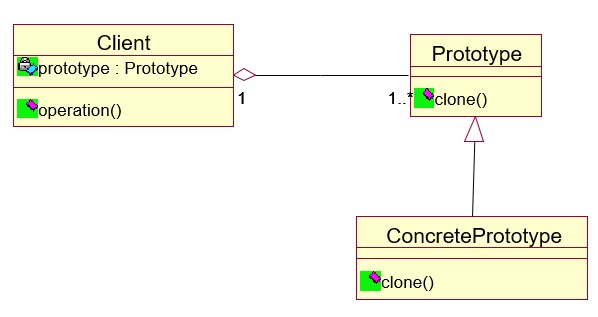
\includegraphics[width=0.55\textwidth]{19_1.jpg}
\end{figure}
以上是第一种形式的原始原型模式,这种形式涉及到三个角色:
\begin{itemize}
  \item 客户端(Client)角色:客户类提出创建对象的请求。
  \item 抽象原型(Prototype)角色:这是一个抽象角色,通常由一个java接口或抽象类实现。此角色给出所有的具体原型类所需的接口。
  \item 具体原型(Concrete Prototype)角色:被复制的对象。此角色需要实现抽象原型角色所要求的接口。
\end{itemize}
%
下面的程序给出了一个示意性的实现,下面是源代码:
\begin{lstlisting}[language=java]
public class Client {
  private Prototype prototype;
  public void operation(Prototype example) {
    Prototype p = (Prototype) example.clone();
  }
}
// 抽象原型角色声明了一个clone()方法
pubilc interface Prototype  extends Cloneable {
   Object clone();
}
// 具体原型角色实现clone()方法
public class ConcretePrototype implements Prototype {
  /* 克隆方法 */
  public Object clone() {
    try {
      return new ConcretePrototype();
    } catch(CloneNotSupportedException e) {
      return null;
    }
  }
}
\end{lstlisting}
%
\textbf{登记式的原型模式}:
\begin{figure}[H]
  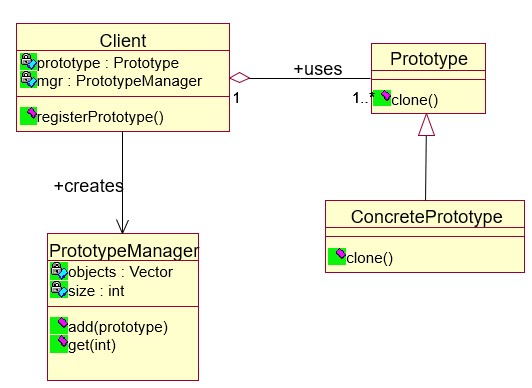
\includegraphics[width=0.50\textwidth]{19_2.jpg}
\end{figure}
该模式有如下的角色:
\begin{itemize}
  \item 客户端(Client)角色:客户端类向原型管理器提出存储或提取对象的请求。
  \item 抽象原型(Prototype)角色:这是一个抽象角色,通常由一个接口或抽象类实现。此角色给出所有的具体原型类所需的接口。
  \item 具体原型(Concrete Prototype)角色:被复制的对象。此角色需要实现抽象的原型角色所要求的接口。
  \item 原型管理器(Prototype Manager)角色:管理记录每一个被创建的对象。
\end{itemize}
%
下面给出一个示意性代码。首先抽象类型角色声明了一个方法,即clone()方法
\begin{lstlisting}[language=java]
public interface Prototype extends Cloneable {
  public Object clone();
}

public class ConcretePrototype implements Prototype {
  string gender;
  public synchronized Object clone() {
    Prototype temp=null;
    temp=new ConcretePrototype ();
    return temp;
  }
}
\end{lstlisting}
%
原型管理器角色保持一个聚集,作为对所有原型对象的登记,这个角色提供必要的方法,供外界增加新的原型对象和取得已经登记过的对象。其源代码如下:
\begin{lstlisting}[language=java]
import java.util.Map;
public class PrototypeManager {
  /* 用来记录原型的编号和原型实例的对应关系 */
  private static Map<String,Prototype> map = new
    HashMap<String, Prototype>();
  /* 私有化构造方法,避免外部创建实例 */
  private PrototypeManager() {  }
  /**
   * 向原型管理器里面添加或是修改某个原型注册
   * @param prototypeId 原型编号
   * @param prototype 原型实例
   */
  public synchronized static void setPrototype(String prototypeId,
    Prototype prototype){
    map.put(prototypeId, prototype);
  }
  /**
   * 获取某个原型编号对应的原型实例
   * @param prototypeId 原型编号
   * @return 原型编号对应的原型实例
   * @throws Exception 如果原型编号对应的实例不存在,
    则抛出异常
   */
  public synchronized static Prototype getPrototype(String prototypeId)
    throws Exception{
    Prototype prototype = map.get(prototypeId);
    if(prototype == null){
      throw new Exception("您希望获取的原型还没有注册或已被销毁");
    }
    return prototype;
  }
}
\end{lstlisting}
%
客户端角色 Client 的源代码如下:
\begin{lstlisting}[language=java]
public class Client {
  try{
    Prototype p1 = new ConcretePrototype();
    // 获取原型来创建对象
    PrototypeManager.setPrototype("p1", p1);
    Prototype p2 = PrototypeManager.getPrototype("p1").clone();
  } catch (Exception e) {  }
}
\end{lstlisting}
\end{document}
